\section{Theorie}
\label{sec:Theorie}

%In knapper Form sind die physikalischen Grundlagen des Versuches, des Messverfahrens, sowie sämtliche %für die Auswertung erforderlichen Gleichungen darzustellen. (Keine Herleitung)

%(eventuell die Aufgaben)

%Der Versuchsaufbau: Beschreibung des Versuchs und der Funktionsweise (mit Skizze/Bild/Foto)

\begin{figure}
    \centering
    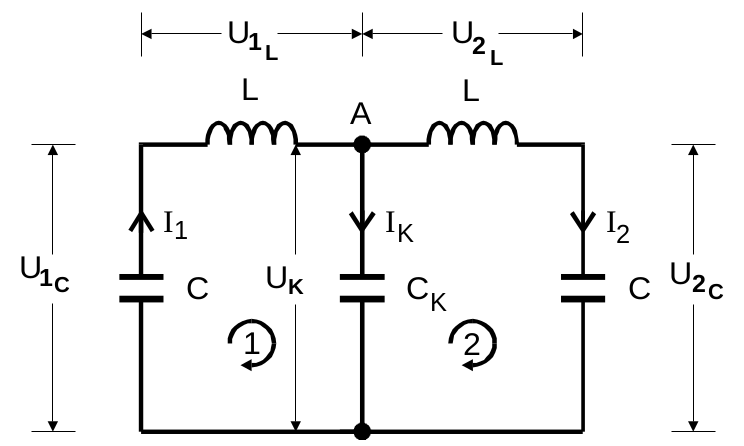
\includegraphics[width=\textwidth/2]{images/schaltung_1.png}
    \caption{Schaltbild der hier beschriebenen gekoppelten Schwingkreise. \cite{V355}}
    \label{fig:schaltung_1}
\end{figure}

Ein elektrischer Schwingkreis ist eine Schaltung bestehend aus einem Widerstand $R$, einer Spule $L$ und einem Kondensator $C$. 
Schwingkreis heißt diese Schaltung, weil sie beschrieben werden kann wie ein harmonischer Oszillator, in dem die Spannungsamplitude und die Stromamplitude gegenphasig hin und her schwingen.
Gekoppelt werden zwei Schwingkreise über einen zusätzlichen Kondensator $C_k$. (siehe \autoref{fig:schaltung_1})
Eine gleiche Resonanzfrequenz der beiden Schwingkreise muss vorausgesetzt sein. 
Dies kann analog angesehen werden wie zwei identische Fadenpendel, welche mit einer Feder gekoppelt sind.

Es gelten die Zusammenhänge von Strom $I$, Spannung $U$, Widerstand $R$, Kapazität $C$ und Induktivität $L$
\begin{align}
    U = RI && U_C = \frac{1}{C} \int I \dif{t} && U_L = L \dot{I}
\end{align}

Nun ergeben für die Ströme $I_1$ und $I_2$ mit den Stromamplituden $I_{1_0}$ und $I_{2_0}$ mithilfe der Kirchhoffschen Regeln die Gleichungen

\begin{align}
    \label{eq:strom}
    I_1(t) &= \frac{1}{2} (I_{1_0} + I_{2_0})\cos(2 \pi \nu _+ t) + \frac{1}{2} (I_{1_0} - I_{2_0})\cos(2 \pi \nu _- t) \\
    I_2(t) &= \frac{1}{2} (I_{1_0} + I_{2_0})\cos(2 \pi \nu _+ t) - \frac{1}{2} (I_{1_0} - I_{2_0})\cos(2 \pi \nu _- t).
\end{align}
Wobei die Frequenzen
\begin{align}
    \label{eq:frequenz+}
    \nu _+ &= \frac{1}{2 \pi \sqrt{L C}} \\
    \label{eq:frequenz-}
    \nu _- &= \frac{1}{2 \pi \sqrt{L \left( \frac{1}{C} + \frac{2}{C_k} \right)^{-1}}}
\end{align}
sind.\cite{V355}

Hieran ist zu sehen, dass das System zwei Fundamentalschwingungen besitzt:
\begin{enumerate}
\item Wenn $I_{1_0} = I_{2_0}$ ist, ist nur der Teil mit $\nu _+$ von Bedeutung und die Schwingkreise schwingen mit gleicher Phase.
\item Wenn $I_{1_0} = - I_{2_0}$ ist, ist nur der Teil mit $\nu _-$ von Bedeutung und die Schwingkreise schwingen mit einem Phasenunterschied von $\pi$.
\end{enumerate}

Wenn nun wie in \autoref{fig:schaltung_2} dargestellt in den Schaltkreis ein Sinusgenerator mit Spannungsamplitude $U_0$ und Frequenz $\omega$ sowie ein Widerstand $R$ eingebaut werden, lässt sich die Stromamplitude $I_2$ des rechten Schwingkreises mit 
\begin{equation}
    \label{eq:stromamplitude}
    I_2 = U_0 \frac{1}{\sqrt{4 \omega^2 C_k^2 R^2 Z(\omega)^2 + \left( \frac{1}{\omega C_k} - \omega C_k Z(\omega)^2 + \omega R^2 C_k \right)^2 }}
\end{equation}
berechnen. Wobei 
\begin{equation}
    Z(\omega) = \omega L - \frac{1}{\omega} \left( \frac{1}{C} + \frac{1}{C_k} \right)
\end{equation}
ist. \cite{V355}
Der Strom durch den Kopplungskondensator ist durch Knotenregel
\begin{equation}
    I_k = I_2 - I_1
\end{equation}
mit 
\begin{equation}
    I_1 = U_0 / R.
\end{equation}
\begin{figure}
    \centering
    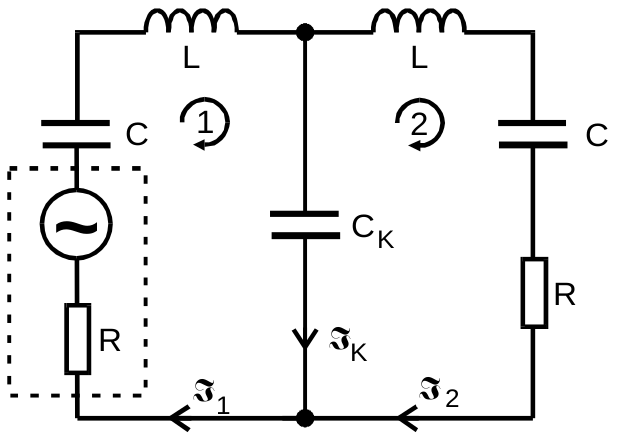
\includegraphics[width=\textwidth/3]{images/schaltung_2.png}
    \caption{Schaltbild der gekoppelten Schwingkreise mit eingebautem Sinusgenerator. \cite{V355}}
    \label{fig:schaltung_2}
\end{figure}

Eine dritte spezielle Schwingung tritt auf wenn bei $t=0$ $I_1 \neq 0$ ist und $I_2 = 0$ ist. Nun ergibt sich eine Schwebung wie in \autoref{fig:schwebung} dargestellt.
\begin{figure}
    \centering
    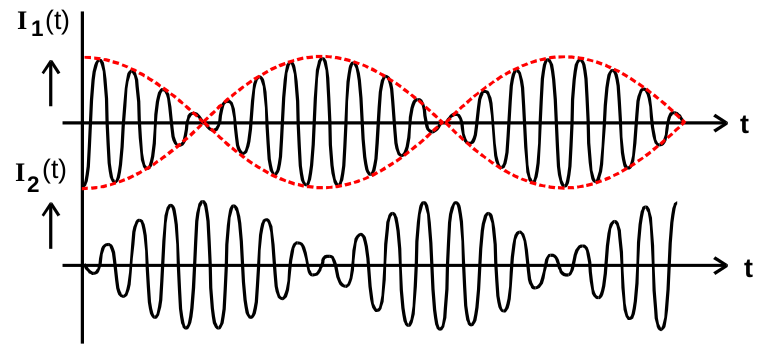
\includegraphics[width=\textwidth/2]{images/schwebung.png}
    \caption{Zeitabhängigkeit der Ströme in den Schwingkreisen im Falle einer Schwebung. \cite{V355}}
    \label{fig:schwebung}
\end{figure}

Hier lässt sich sehen, dass es einen periodischen Energieaustausch zwischen den Schwingkreisen gibt. 
Wobei nun $\frac{1}{2} (\nu _+ + \nu _-)$ die Schwingungsfrequenz und $\nu _- - \nu _+$ die Schwebungsfrequenz ist.\cite{V355}

Also ist 
\begin{equation}
    \label{eq:extrema}
    N \coloneq \frac{1}{2} \cdot \frac{ \nu _+ + \nu _-}{\nu _- - \nu _+}
\end{equation}
die Anzahl der Maxima der Schwingung innerhalb eines Nulldurchgangs der Schwebung.